\section{Results}

\subsection{Preselection}
\DIFdelbegin \DIFdel{Performance scores of various estimators elaborated }\DIFdelend \DIFaddbegin

    \DIFadd{For the estimators listed }\DIFaddend in Table~\ref{table:AImethods}\DIFdelbegin \DIFdel{are presented }\DIFdelend \DIFaddbegin \DIFadd{, we presented performance score }\DIFaddend in Table~\ref{table:regression} for \DIFdelbegin \DIFdel{the regression analyses and presented }\DIFdelend \DIFaddbegin \DIFadd{regression analysis and }\DIFaddend in Table~\ref{table:classification} for \DIFdelbegin \DIFdel{the classification analyses}\DIFdelend \DIFaddbegin \DIFadd{classification analysis}\DIFaddend . The results were obtained using the default \DIFdelbegin \DIFdel{hyper-parameters. Each estimator demonstrated its own characteristic behavior
and, }\DIFdelend \DIFaddbegin \DIFadd{hyperparameters. }\DIFaddend \gls{RF}, \gls{ET}, \gls{KN}, \DIFdelbegin %DIFDELCMD < \gls{SV}%%%
\DIFdelend \DIFaddbegin \gls{SVM}\DIFaddend , and \gls{MLP} estimators predicted the performance metrics with significantly higher accuracy than the others. Even without \DIFdelbegin \DIFdel{optimizing the hyper-parameters of the estimators, $R^2$ }\DIFdelend \DIFaddbegin \DIFadd{hyperparameter optimization, }\gls{R2} \DIFaddend scores of these five estimators \DIFdelbegin \DIFdel{range }\DIFdelend \DIFaddbegin \DIFadd{ranged }\DIFaddend from 90 to 98\% for regression and from 92 to 96\% for classification. This implies that the \DIFdelbegin \DIFdel{models trained }\DIFdelend \DIFaddbegin \DIFadd{trained models }\DIFaddend by these estimators will have very low variance. The \gls{ET} regressor most accurately predicted the performance metrics while the \DIFdelbegin %DIFDELCMD < \gls{SV} %%%
\DIFdelend \DIFaddbegin \gls{SVM} \DIFaddend classifier was superior to \DIFdelbegin \DIFdel{other
estimators in classifying the design labels defined as reactor type, spectrum,
criticality and feedback}\DIFdelend \DIFaddbegin \DIFadd{the others in classifying designs}\DIFaddend .

    In general, the linear methods (i.e., \DIFdelbegin \DIFdel{SGD, R, EN, L, LL, P, and Log) yield lower a fit \_score (and thus higher errors ) }\DIFdelend \DIFaddbegin \gls{SGD}\DIFadd{, }\gls{R}\DIFadd{, }\gls{EN}\DIFadd{, }\gls{L}\DIFadd{, }\gls{LL}\DIFadd{, }\gls{P}\DIFadd{, and }\gls{Log}\DIFadd{) yielded lower fit scores and higher errors }\DIFaddend with respect to the non-linear methods such as ensemble, \gls{SVM}, and \gls{ANN}. These results clearly imply that \DIFdelbegin \DIFdel{the
}\DIFdelend linear methods are not quite enough to design a nuclear reactor and thus in predicting its performance metrics. Like \DIFdelbegin \DIFdel{the }\DIFdelend linear methods, the \DIFdelbegin \DIFdel{Naive Bayes
}\DIFdelend \DIFaddbegin \gls{NB} \DIFaddend classification methods such as \DIFdelbegin \DIFdel{GNB and BNB }\DIFdelend \DIFaddbegin \gls{GNB} \DIFadd{and }\gls{BNB} \DIFaddend seem inappropriate due to the suboptimal performance scores. \DIFaddbegin \DIFadd{This is because these methods such as linear and }\gls{NB} \DIFadd{are not sufficient to fit the training dataset (leading to underfitting) into a linear function due to the higher degree interdependencies of our feature parameters. }\DIFaddend In addition to this, the \gls{RF}, \gls{DT}, \DIFdelbegin \DIFdel{B, and AB regressors and classifiers, have }\DIFdelend \DIFaddbegin \gls{B}\DIFadd{, and }\gls{AB} \DIFadd{estimators, gave }\DIFaddend similar results, except for fit score values, as they use the same base estimator (\DIFdelbegin \DIFdel{decision tree}\DIFdelend \DIFaddbegin \gls{DT}\DIFaddend ) in training. Likewise, the \DIFdelbegin \DIFdel{LP classifier produces }\DIFdelend \DIFaddbegin \gls{LP} \DIFadd{classifier produced }\DIFaddend the same results with the \DIFdelbegin %DIFDELCMD < \gls{SV}
%DIFDELCMD < %%%
\DIFdelend \DIFaddbegin \gls{SVM} \DIFaddend classifier due to the use of the same kernel ($rbf$). In \DIFdelbegin \DIFdel{the }\DIFdelend regression analysis, the \gls{ET} regressor has the lowest \gls{MAE} and \gls{MSE} scores while the \DIFdelbegin \DIFdel{R }\DIFdelend \DIFaddbegin \gls{R} \DIFaddend regressor has the highest scores.

    As to the classification, the \DIFdelbegin %DIFDELCMD < \gls{SV}  %%%
\DIFdelend \DIFaddbegin \gls{SVM} \DIFaddend classifier has the lowest \gls{HL} and \gls{LRL} scores while the \DIFdelbegin \DIFdel{Perceptron }\DIFdelend \DIFaddbegin \gls{P} \DIFaddend classifier has the highest scores. \DIFdelbegin \DIFdel{Furthermore}\DIFdelend \DIFaddbegin \DIFadd{Briefly}\DIFaddend , any design can be classified with \DIFdelbegin \DIFdel{a small fraction of }\DIFdelend \DIFaddbegin \DIFadd{high precision ($>$ 95\%) and very few }\DIFaddend incorrectly predicted labels (\DIFaddbegin \DIFadd{false neagtive plus false positive: }\DIFaddend $<$ 5\%)\DIFdelbegin \DIFdel{and a high precision ($>$ 95\%)}\DIFdelend , leading to an opportunity for an accurate prediction of reactor design even without making any regression analysis.

    \DIFdelbegin \DIFdel{From the results of the preselection phase}\DIFdelend \DIFaddbegin \DIFadd{On the whole}\DIFaddend , five estimators (i.e., \gls{RF}, \gls{ET}, \gls{KN}, \DIFdelbegin %DIFDELCMD < \gls{SV}%%%
\DIFdelend \DIFaddbegin \gls{SVM}\DIFaddend , and \gls{MLP}) \DIFdelbegin \DIFdel{satisfying }\DIFdelend \DIFaddbegin \DIFadd{that satisfy }\DIFaddend a score of more than 90\% in \DIFdelbegin \DIFdel{the $R^2$ and fit score values seem }\DIFdelend \DIFaddbegin \gls{R2} \DIFadd{and fit scores appear to be }\DIFaddend suitable for the subsequent stage of \DIFdelbegin \DIFdel{the }\DIFdelend calculations. Among the selected estimators, \DIFdelbegin \DIFdel{despite its worst fit score
value, the }%DIFDELCMD < \gls{SV} %%%
\DIFdelend \DIFaddbegin \DIFadd{the }\gls{SVM} \DIFaddend regressor interestingly shows the second-best performance right after the \gls{ET} regressor \DIFaddbegin \DIFadd{despite its worst fit score}\DIFaddend . In fact, \DIFdelbegin \DIFdel{all }\DIFdelend \DIFaddbegin \DIFadd{as }\DIFaddend the scores of the \DIFdelbegin \DIFdel{five selected
}\DIFdelend \DIFaddbegin \DIFadd{best performing }\DIFaddend estimators are very close to each other\DIFdelbegin \DIFdel{and }\DIFdelend \DIFaddbegin \DIFadd{, }\DIFaddend at this point\DIFaddbegin \DIFadd{, }\DIFaddend it is not easy to distinguish which estimator is \DIFaddbegin \DIFadd{the }\DIFaddend best. Therefore, in the following section, the \DIFaddbegin \DIFadd{current }\DIFaddend scores of these \DIFdelbegin \DIFdel{five }\DIFdelend estimators are further improved by tuning their \DIFdelbegin \DIFdel{hyper-parameters}\DIFdelend \DIFaddbegin \DIFadd{hyperparameters and investigating their learning curves}\DIFaddend .

%%%%%%%%%%%%%%%%%%%%%%%%%%%%%%%%%%%%%%%%
\begin{landscape}
	\begin{table}[ht!]
		\centering
		\caption{Performance scores \DIFdelbeginFL \DIFdelFL{for various }\DIFdelendFL \DIFaddbeginFL \DIFaddFL{of the studied }\DIFaddendFL regression methods}
		\begin{tabular}{l>{\columncolor[gray]{0.9}}l>{\columncolor[gray]{0.9}}
				l>{\columncolor[gray]{0.9}}l>{\columncolor[gray]{0.9}}
				l>{\columncolor[gray]{0.9}}lllllllllllllllllllllllllll}
			\hline
			& \textbf{\gls{RF}} & \textbf{\gls{ET}} & \textbf{\gls{KN}} &
			\textbf{\DIFdelbeginFL %DIFDELCMD < \gls{SV}%%%
\DIFdelendFL \DIFaddbeginFL \gls{SVM}\DIFaddendFL } & \textbf{\gls{MLP}} & \textbf{\gls{DT}} & \textbf{GB} &
			\textbf{B} & \textbf{AB} & \textbf{SGD} & \textbf{R} & \textbf{EN} &
			\textbf{L} & \textbf{LL} \\
			\hline
			fit \DIFdelbeginFL \DIFdelFL{$\_$}\DIFdelendFL score & 1.00 & 1.00 	& 0.99  & 0.96 	& 0.99  & 1.00 & 0.97 & 1.00
			& 0.78	& 0.54 	& 0.73 	& 0.70 	& 0.69 	& 0.55 \\
			EVR  & 0.90 & 0.98 & 0.97 & 0.98 	& 0.95  & 0.90 &
			0.89 & 0.90 & 0.54	& 0.38 & 0.37 & 0.46 & 0.25 & 0.38 \\
			\gls{MAE} & 1.27 & 0.35	& 0.57  & 0.54 	& 0.87  & 1.28 &
			1.72 & 1.27 & 3.36 & 4.77 & 4.78 & 4.60 & 4.77 	& 4.77	\\
			\gls{MSE} & 7.60 & 0.62 & 1.61 & 1.45 & 2.97 & 7.71 & 12.99
			& 7.60 & 38.85 & 82.73	& 82.94	& 77.95	& 81.94	& 82.95	\\
			R$^2$ & 0.90 & 0.98 & 0.97 & 0.98 & 0.95  & 0.90 & 0.89 & 0.90 &
			0.00 & 0.23 & 0.22 & 0.35 & 0.07 & 0.23	\\
			\hline
		\end{tabular}
		\label{table:regression}
	\end{table}
	%%%%%%%%%%%%%%%%%%%%%%%%%%%%%%%%%%%%%%%%
	\begin{table}[ht!]
		\caption{Performance scores \DIFdelbeginFL \DIFdelFL{for various }\DIFdelendFL \DIFaddbeginFL \DIFaddFL{of the studied }\DIFaddendFL classification methods}
		\begin{tabular}{l>{\columncolor[gray]{0.9}}l>{\columncolor[gray]{0.9}}
				l>{\columncolor[gray]{0.9}}l>{\columncolor[gray]{0.9}}
				l>{\columncolor[gray]{0.9}}llllllllllllllllll}
			\hline
			& \textbf{\gls{RF}} & \textbf{\gls{ET}} & \textbf{\gls{KN}}	&
			\textbf{\DIFdelbeginFL %DIFDELCMD < \gls{SV}%%%
\DIFdelendFL \DIFaddbeginFL \gls{SVM}\DIFaddendFL }   & \textbf{\gls{MLP}}& \textbf{\gls{DT}} &
			\textbf{\DIFdelbeginFL \DIFdelFL{B}\DIFdelendFL \DIFaddbeginFL \gls{B}\DIFaddendFL } &
			\textbf{\DIFdelbeginFL \DIFdelFL{LP}\DIFdelendFL \DIFaddbeginFL \gls{LP}\DIFaddendFL } & \textbf{\DIFdelbeginFL \DIFdelFL{GB}\DIFdelendFL \DIFaddbeginFL \gls{GB}\DIFaddendFL }  & \textbf{\DIFdelbeginFL \DIFdelFL{AB}\DIFdelendFL \DIFaddbeginFL \gls{AB}\DIFaddendFL } &
			\textbf{\DIFdelbeginFL \DIFdelFL{SGD}\DIFdelendFL \DIFaddbeginFL \gls{SGD}\DIFaddendFL }	& \textbf{\DIFdelbeginFL \DIFdelFL{R}\DIFdelendFL \DIFaddbeginFL \gls{R}\DIFaddendFL } &
			\textbf{\DIFdelbeginFL \DIFdelFL{GNB}\DIFdelendFL \DIFaddbeginFL \gls{GNB}\DIFaddendFL }  & \textbf{\DIFdelbeginFL \DIFdelFL{BNB}\DIFdelendFL \DIFaddbeginFL \gls{BNB}\DIFaddendFL }& \textbf{\DIFdelbeginFL \DIFdelFL{P}\DIFdelendFL \DIFaddbeginFL \gls{P}\DIFaddendFL }&
			\textbf{\DIFdelbeginFL \DIFdelFL{Log}\DIFdelendFL \DIFaddbeginFL \gls{Log}\DIFaddendFL }\\
			\hline
			fit \DIFdelbeginFL \DIFdelFL{$\_$}\DIFdelendFL score  	& 1.00 	& 1.00 	& 0.91 	& 0.90 	& 0.90 	& 1.00 	& 0.98 	& 0.90
			& 0.88 & 0.84 	& 0.61 	& 0.65 	& 0.64 	& 0.55 	& 0.45 	& 0.68\\
			\DIFdelbeginFL \DIFdelFL{AP }\DIFdelendFL \DIFaddbeginFL \gls{AP} \DIFaddendFL & 0.90 	& 0.93 	& 0.92 	& 0.95 	& 0.96 	& 0.90 	&
			0.90 	& 0.96 	& 0.91 & 0.90 	& 0.80 	& 0.69 	& 0.78 	& 0.52 	& 0.77 	& 0.81\\
			\gls{HL} & 0.05 	& 0.04 	& 0.04 	& 0.03 	& 0.04 	& 0.05 	&
			0.05 	& 0.04 	& 0.05 & 0.06 	& 0.17 	& 0.18 	& 0.13 	& 0.18 	& 0.22 	& 0.17\\
			\DIFdelbeginFL \DIFdelFL{LRAPS }\DIFdelendFL \DIFaddbeginFL \gls{LRAPS} \DIFaddendFL & 0.94 	& 0.95 	& 0.95 	& 0.96 	& 0.96 	& 0.94 	& 0.94
			& 0.95 	& 0.94 & 0.93 	& 0.81 	& 0.81 	& 0.86 	& 0.82 	& 0.77 	& 0.82\\
			\gls{LRL} & 0.09 	& 0.07 	& 0.07 	& 0.06 	& 0.06 	& 0.09 	&
			0.09 	& 0.06 	& 0.08 & 0.09 	& 0.27 	& 0.28 	& 0.21 	& 0.27 	& 0.34 	& 0.27\\
			\DIFdelbeginFL \DIFdelFL{ROCAUC }\DIFdelendFL \DIFaddbeginFL \gls{ROCAUC} \DIFaddendFL & 0.92 	& 0.94 	& 0.94 	& 0.96 	& 0.95 	& 0.92 	&
			0.92 	&
			0.92 	& 0.93 & 0.93 	& 0.79 	& 0.70 	& 0.87 	& 0.60 	& 0.75 	& 0.77\\
			\hline
		\end{tabular}
		\label{table:classification}
	\end{table}
\end{landscape}
%%%%%%%%%%%%%%%%%%%%%%%%%%%%%%%%%%%%%%%%

\subsection{\DIFdelbegin \DIFdel{Hyper-parameters }\DIFdelend \DIFaddbegin \DIFadd{Hyperparameters }\DIFaddend optimization and learning curve}
\DIFaddbegin

    \DIFaddend We applied two distinct methods to the \DIFdelbegin \DIFdel{selected }\DIFdelend estimators to improve their performance. The first method, expected to have an impact on the \DIFdelbegin \DIFdel{R$^2$ }\DIFdelend \DIFaddbegin \gls{R2} \DIFaddend scores, prediction errors\DIFaddbegin \DIFadd{, }\DIFaddend and thus cross-validation results, \DIFdelbegin \DIFdel{relies on finding an optimal sample size . As an
illustration}\DIFdelend \DIFaddbegin \DIFadd{aims to find an optimal size for the training dataset. For this}\DIFaddend , Figure~\ref{fig:lc} demonstrates the \DIFdelbegin \DIFdel{learning curves of }\DIFdelend \DIFaddbegin \DIFadd{estimator's learning curves for }\DIFaddend the (U-Th)F$_4$-NaF-BeF$_2$ fuel-salt pair \DIFdelbegin \DIFdel{for the selected regressors }\DIFdelend from the viewpoint of \DIFdelbegin \DIFdel{the R$^2$ score and for the selected classifiers from the viewpoint
of }\DIFdelend \DIFaddbegin \gls{R2} \DIFadd{score in regression and }\DIFaddend multi-label classification accuracy \DIFdelbegin \DIFdel{score (f1\_samples)}\DIFdelend \DIFaddbegin \DIFadd{in classification}\DIFaddend .

    \DIFaddbegin \DIFadd{At first look, the }\gls{MLP} \DIFadd{and }\gls{SVM} \DIFadd{predictive models do not require more data since the training and cross-validation scores converge together. On the contrary, the }\gls{RF}\DIFadd{, }\gls{ET} \DIFadd{and }\gls{KN} \DIFadd{models require more data as their training scores are much higher than their cross-validation scores.
}

    \DIFaddend From all the learning curves\DIFdelbegin \DIFdel{of fuel-salt pairs, random forest (}\DIFdelend \DIFaddbegin \DIFadd{, the }\DIFaddend \gls{RF}\DIFdelbegin \DIFdel{), extra-trees (}\DIFdelend \DIFaddbegin \DIFadd{, }\DIFaddend \gls{ET}\DIFdelbegin \DIFdel{), multi-layer perceptron (}\DIFdelend \DIFaddbegin \DIFadd{, }\DIFaddend \gls{MLP}\DIFdelbegin \DIFdel{), and support vector (}%DIFDELCMD < \gls{SV}%%%
\DIFdel{)
regressors require a sample }\DIFdelend \DIFaddbegin \DIFadd{, and }\gls{SVM} \DIFadd{models require a training }\DIFaddend size in the range of 32000 and 40000 in which the curves level off to \DIFdelbegin \DIFdel{the R$^2$ }\DIFdelend \DIFaddbegin \DIFadd{a }\gls{R2} \DIFaddend score of 0.99 \DIFdelbegin \DIFdel{and
k-nearest neighbors (}\DIFdelend \DIFaddbegin \DIFadd{whereas the }\DIFaddend \gls{KN} \DIFdelbegin \DIFdel{) requires a }\DIFdelend \DIFaddbegin \DIFadd{model requires }\DIFaddend sample size more than 40000. A similar situation was observed in the \DIFdelbegin \DIFdel{learning curves of the
classifiers}\DIFdelend \DIFaddbegin \DIFadd{classifiers' learning curves}\DIFaddend . As a result, we \DIFdelbegin \DIFdel{have }\DIFdelend decided to use about forty thousand samples for each fuel-salt pair. In other words, for nine fuel-salt pairs, we generated around three hundred thousand samples in total. In the second method, we obtained \DIFdelbegin \DIFdel{the optimum
hyper-parameters }\DIFdelend \DIFaddbegin \DIFadd{optimal hyperparameters }\DIFaddend of the estimators tabulated in Table~\ref{table:hyper}. \DIFdelbegin \DIFdel{In the
table, the parameters not listed had optimal }\DIFdelend \DIFaddbegin \DIFadd{Parameters not listed in the table are at their }\DIFaddend default values and \DIFdelbegin \DIFdel{required no tuning}\DIFdelend \DIFaddbegin \DIFadd{do not need optimization}\DIFaddend .

%%%%%%%%%%%%%%%%%%%%%%%%%%%%%%%%%%%%%%%
    \begin{figure}[ht!]
    	\begin{center}
    		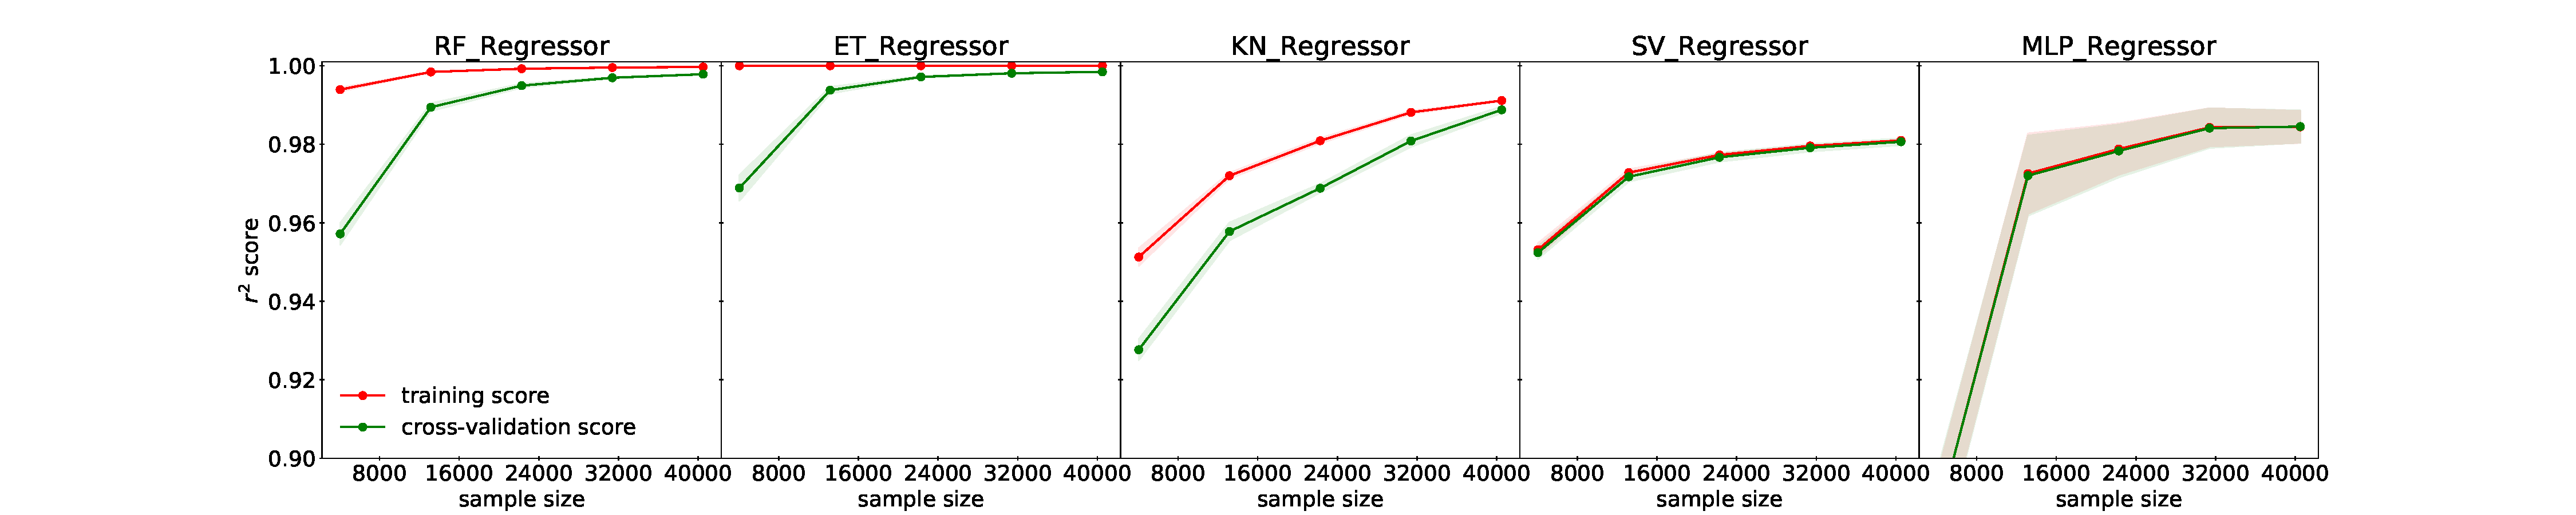
\includegraphics[trim=200 0 200 0, clip,
    		width=\textwidth]{images/regressors_learning_curves.pdf}

    		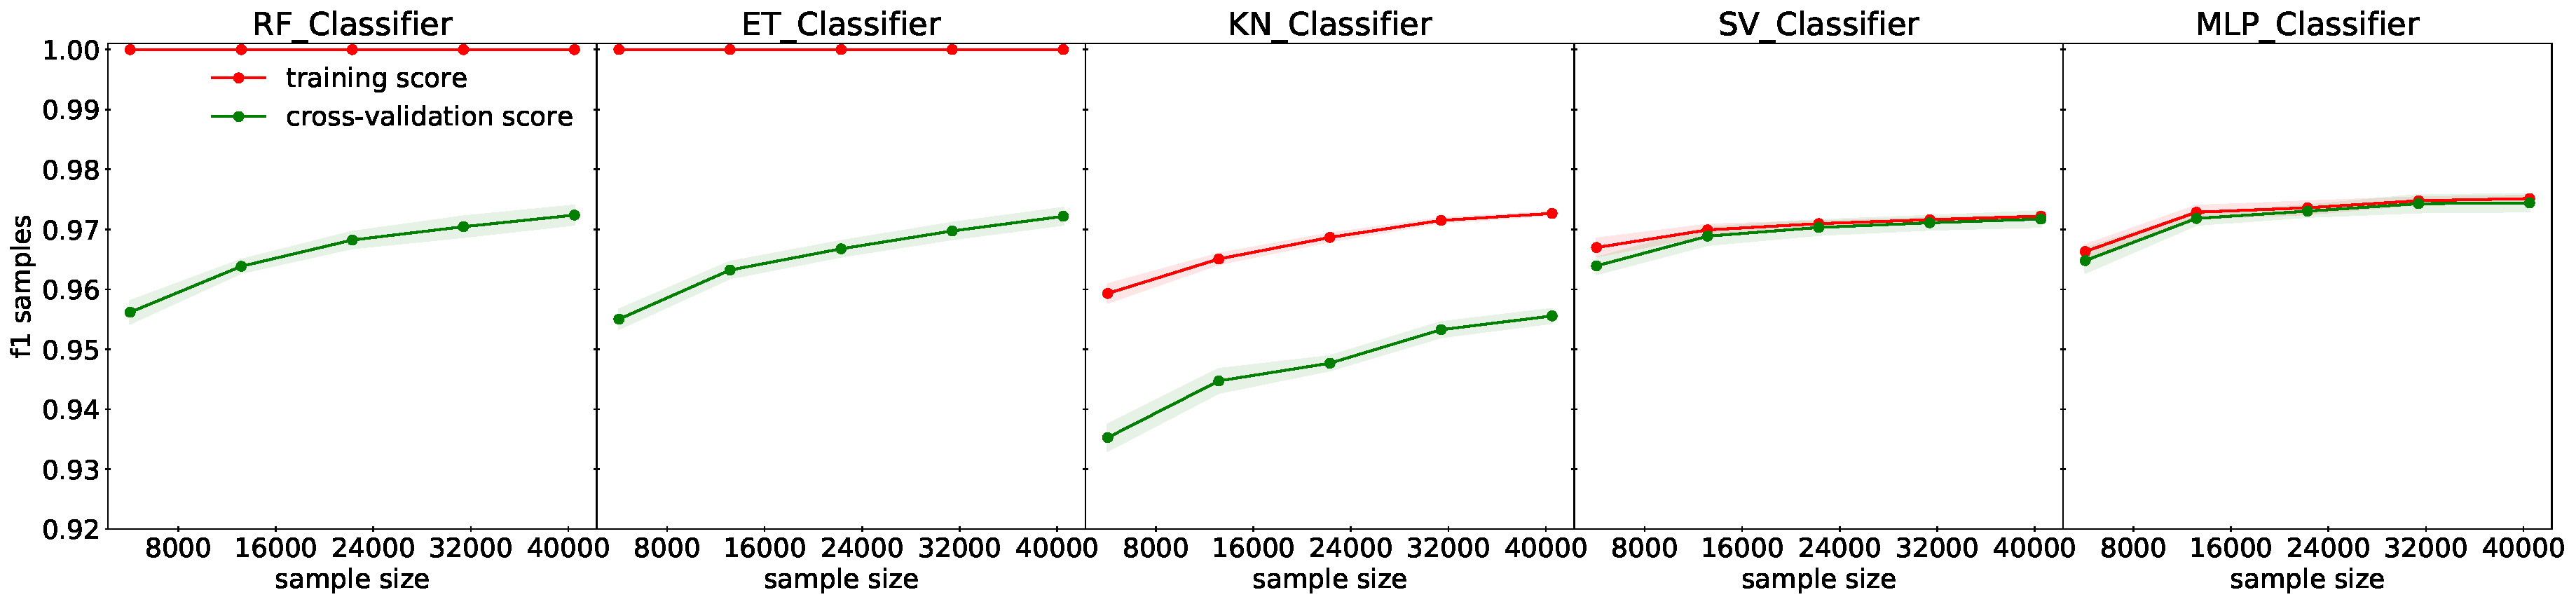
\includegraphics[width=\textwidth]{images/classifiers_learning_curves.pdf}
    	\end{center}
    	\caption{Learning curves of the selected estimators\DIFaddbeginFL \DIFaddFL{. Solid lines represent mean scores, while the shaded areas around lines represent the standard deviation of the mean due to error.}\DIFaddendFL }
    	\label{fig:lc}
    \end{figure}
%%%%%%%%%%%%%%%%%%%%%%%%%%%%%%%%%%%%%%%%
%%%%%%%%%%%%%%%%%%%%%%%%%%%%%%%%%%%%%%%%
\begin{table}[ht!]
	\centering
	\caption{Optimal \DIFdelbeginFL \DIFdelFL{hyper-parameters }\DIFdelendFL \DIFaddbeginFL \DIFaddFL{hyperparameters }\DIFaddendFL of the selected estimators}
	\DIFdelbeginFL %DIFDELCMD < \begin{tabular}{ll}
%DIFDELCMD < 		%%%
\DIFdelendFL \DIFaddbeginFL \begin{tabular}{l p{0.8\linewidth}}
%		\DIFaddendFL \hline
		\textbf{Method} & \textbf{Parameters  (Regressor/Classifier)} \\
        \hline
		\gls{RF} & \DIFdelbeginFL \DIFdelFL{max$\_$}\DIFdelendFL \DIFaddbeginFL \DIFaddFL{maximum }\DIFaddendFL features: None/None, \DIFdelbeginFL \DIFdelFL{n$\_$estimators}\DIFdelendFL \DIFaddbeginFL \DIFaddFL{number of trees}\DIFaddendFL : 400/400, \DIFdelbeginFL %DIFDELCMD < \\
%DIFDELCMD < 		                & %%%
\DIFdelFL{min$\_$samples$\_$leaf}\DIFdelendFL \DIFaddbeginFL \DIFaddFL{minimum number of samples}\DIFaddendFL : 7/7                 \\
		\gls{ET} & \DIFdelbeginFL \DIFdelFL{max$\_$}\DIFdelendFL \DIFaddbeginFL \DIFaddFL{maximum }\DIFaddendFL features: None/None, \DIFdelbeginFL \DIFdelFL{n$\_$estimators}\DIFdelendFL \DIFaddbeginFL \DIFaddFL{number of trees}\DIFaddendFL : 800/800, \DIFdelbeginFL %DIFDELCMD < \\
%DIFDELCMD < 		                & %%%
\DIFdelFL{min$\_$samples$\_$leaf}\DIFdelendFL \DIFaddbeginFL \DIFaddFL{minimum number of samples}\DIFaddendFL : 1/7, \DIFaddbeginFL \DIFaddFL{quality }\DIFaddendFL criterion: -/gini    \\
		\gls{KN} & \DIFdelbeginFL \DIFdelFL{weights}\DIFdelendFL \DIFaddbeginFL \DIFaddFL{weight function}\DIFaddendFL : distance/distance, \DIFdelbeginFL \DIFdelFL{n$\_$}\DIFdelendFL \DIFaddbeginFL \DIFaddFL{number of }\DIFaddendFL neighbors: 7/44, \DIFdelbeginFL %DIFDELCMD < \\
%DIFDELCMD < 		                & %%%
\DIFdelendFL \DIFaddbeginFL \DIFaddFL{distance }\DIFaddendFL metric: manhattan/manhattan, leaf \DIFdelbeginFL \DIFdelFL{$\_$}\DIFdelendFL size: 136/200  \\
		\DIFdelbeginFL %DIFDELCMD < \gls{SV}        %%%
\DIFdelendFL \DIFaddbeginFL \gls{SVM} \DIFaddendFL & kernel \DIFaddbeginFL \DIFaddFL{type}\DIFaddendFL : rbf/poly, \DIFaddbeginFL \DIFaddFL{polynomial }\DIFaddendFL degree: -/3, \DIFdelbeginFL \DIFdelFL{gamma}\DIFdelendFL \DIFaddbeginFL \DIFaddFL{kernel coefficient}\DIFaddendFL : auto/scale, \DIFdelbeginFL %DIFDELCMD < \\
%DIFDELCMD < 		                & %%%
\DIFdelendFL epsilon: 0.1/-, \DIFdelbeginFL \DIFdelFL{C}\DIFdelendFL \DIFaddbeginFL \DIFaddFL{regularization parameter}\DIFaddendFL : 3.4/1.2, \DIFdelbeginFL \DIFdelFL{tol}\DIFdelendFL \DIFaddbeginFL \DIFaddFL{stopping criterion}\DIFaddendFL : 1e-5 \\
		\gls{MLP} & activation \DIFaddbeginFL \DIFaddFL{function}\DIFaddendFL : relu/tanh, hidden \DIFdelbeginFL \DIFdelFL{$\_$layer$\_$sizes}\DIFdelendFL \DIFaddbeginFL \DIFaddFL{layers}\DIFaddendFL : 1000/250, \DIFdelbeginFL %DIFDELCMD < \\
%DIFDELCMD < 		                & %%%
\DIFdelFL{max$\_$iter}\DIFdelendFL \DIFaddbeginFL \DIFaddFL{maximum iterations}\DIFaddendFL : 1e4/1e4, tol: 1e-5, solver: adam/sgd, \DIFdelbeginFL %DIFDELCMD < \\
%DIFDELCMD < 		                & %%%
\DIFdelFL{learning $\_$}\DIFdelendFL \DIFaddbeginFL \DIFaddFL{learning }\DIFaddendFL rate: adaptive/constant       \\ \hline
	\end{tabular}
	\label{table:hyper}
\end{table}

\subsection{Final Estimators}
\DIFaddbegin

    \DIFaddend After performing the \DIFdelbegin \DIFdel{hyper-parameter }\DIFdelend \DIFaddbegin \DIFadd{hyperparameter }\DIFaddend optimization and learning curve \DIFdelbegin \DIFdel{assessments, we calculated }\DIFdelend \DIFaddbegin \DIFadd{assessment, we evaluated }\DIFaddend the final scores of the selected estimators and listed them in Table~\ref{table:finalreg} and ~\ref{table:finalclf}. At a \DIFdelbegin \DIFdel{quick
glance, }\DIFdelend \DIFaddbegin \DIFadd{glance, we saw that }\DIFaddend there is a slight enhancement in the performance scores of all regressors\DIFaddbegin \DIFadd{, }\DIFaddend except for the scores of \DIFaddbegin \DIFadd{the }\DIFaddend \gls{MLP} \DIFdelbegin \DIFdel{explicitly exhibiting a strong hyper-parameter dependency. On the other hand, optimization failed to improve classifier performance}\DIFdelend \DIFaddbegin \DIFadd{regressor that exhibits a strong hyperparameter dependency. However, the hyperparameter optimization did not improve the scores of the classifiers}\DIFaddend . With the optimized \DIFdelbegin \DIFdel{hyper-parameters and sample size in training}\DIFdelend \DIFaddbegin \DIFadd{hyperparameters and data size in the training dataset}\DIFaddend , the \gls{ET}, \DIFdelbegin %DIFDELCMD < \gls{SV}%%%
\DIFdelend \DIFaddbegin \gls{SVM}\DIFaddend , and \gls{MLP} regressors \DIFdelbegin \DIFdel{now predict
}\DIFdelend \DIFaddbegin \DIFadd{predicted }\DIFaddend performance metrics with a higher \DIFdelbegin \DIFdel{R$^2$ and lower mean absolute error (MAE)
compared to the }\DIFdelend \DIFaddbegin \gls{R2} \DIFadd{and lower }\gls{MAE} \DIFadd{compared to their }\DIFaddend preselection scores.

    \DIFdelbegin \DIFdel{Likewise, the }%DIFDELCMD < \gls{SV}  %%%
\DIFdelend \DIFaddbegin \DIFadd{On the other hand, the }\gls{SVM} \DIFaddend and \gls{MLP} classifiers \DIFdelbegin \DIFdel{label }\DIFdelend \DIFaddbegin \DIFadd{labeled }\DIFaddend the design attributes \DIFdelbegin \DIFdel{,
providing a higher average precision (AP) and lower label ranking loss (LRL).
The }%DIFDELCMD < \gls{MLP} %%%
\DIFdel{and }%DIFDELCMD < \gls{ET} %%%
\DIFdel{methods demonstrate the lowest errors }\DIFdelend \DIFaddbegin \DIFadd{with the highest }\gls{AP} \DIFadd{and lowest }\gls{LRL} \DIFadd{scores }\DIFaddend relative to the other estimators\DIFdelbegin \DIFdel{and one accordingly promising candidates for the subsequent
phase of this study. To select the right estimator(s) }\DIFdelend \DIFaddbegin \DIFadd{. Nonetheless, the others are also suitable as all the scores are very close to each other. As the scores did not give us sufficient information about determining the right estimator }\DIFaddend for the next phase, \DIFdelbegin \DIFdel{the
}\DIFdelend \DIFaddbegin \DIFadd{we investigated }\DIFaddend cross-validation plots and multi-label confusion matrices \DIFaddbegin \DIFadd{on the basis }\DIFaddend of each performance metric (i.e., $k_{\infty}$, $\varsigma$, $\phi_{fast}$)\DIFdelbegin \DIFdel{must be investigated}\DIFdelend .

%%%%%%%%%%%%%%%%%%%%%%%%%%%%%%%%%%%%%%%%
    \begin{table}[ht!]
    	\centering
    	\caption{\DIFdelbeginFL \DIFdelFL{Performance }\DIFdelendFL \DIFaddbeginFL \DIFaddFL{Final performance }\DIFaddendFL scores \DIFdelbeginFL \DIFdelFL{for }\DIFdelendFL \DIFaddbeginFL \DIFaddFL{of }\DIFaddendFL the selected regressors}
    	\begin{tabular}{lllll>{\columncolor[gray]{0.9}}l}
    		\hline
    		& \textbf{\gls{RF}}  & \textbf{\gls{ET}}  & \textbf{\gls{KN}} &
    		\textbf{\DIFdelbeginFL %DIFDELCMD < \gls{SV}%%%
\DIFdelendFL \DIFaddbeginFL \gls{SVM}\DIFaddendFL }   & \textbf{\gls{MLP}} \\
    		\hline
    		\DIFdelbeginFL \DIFdelFL{$fit$\_$score$  }\DIFdelendFL \DIFaddbeginFL \DIFaddFL{fit score  }\DIFaddendFL & 1.00 	& 1.00 & 1.00 & 0.97  & 1.00 \\
    		\DIFdelbeginFL \DIFdelFL{EVR }\DIFdelendFL \DIFaddbeginFL \gls{EVR} \DIFaddendFL & 0.94 & 0.99 & 0.99 & 0.96 & 1.00 \\
    		\gls{MAE} & 1.07 & 0.28 & 0.41 & 0.37 & 0.23 \\
    		\gls{MSE} & 5.52 & 0.41 & 0.83 & 0.44 & 0.24 \\
    		R$^2$ & 0.94 & 0.99 & 0.98 & 0.96 & 1.00 \\
    		\hline
    	\end{tabular}
    	\label{table:finalreg}
    \end{table}
%%%%%%%%%%%%%%%%%%%%%%%%%%%%%%%%%%%%%%%%
    \begin{table}[ht!]
    	\centering
    	\caption{\DIFdelbeginFL \DIFdelFL{Performance }\DIFdelendFL \DIFaddbeginFL \DIFaddFL{Final performance }\DIFaddendFL scores \DIFdelbeginFL \DIFdelFL{for }\DIFdelendFL \DIFaddbeginFL \DIFaddFL{of }\DIFaddendFL the selected classifiers}
    	\begin{tabular}{lllll>{\columncolor[gray]{0.9}}l}
    		\hline
    		& \textbf{\gls{RF}} & \textbf{\gls{ET}}  & \textbf{\gls{KN}} &
    		\textbf{\DIFdelbeginFL %DIFDELCMD < \gls{SV}%%%
\DIFdelendFL \DIFaddbeginFL \gls{SVM}\DIFaddendFL }  & \textbf{\gls{MLP}} \\
    		\hline
    		\DIFdelbeginFL \DIFdelFL{$fit$\_$score$  }\DIFdelendFL \DIFaddbeginFL \DIFaddFL{fit score  }\DIFaddendFL & 0.93 & 1.00 & 1.00  & 0.89 & 0.90 \\
    		\DIFdelbeginFL \DIFdelFL{AP }\DIFdelendFL \DIFaddbeginFL \gls{AP} \DIFaddendFL & 0.92 & 0.94 & 0.95  & 0.96 & 0.97  \\
    		\gls{HL} & 0.04 & 0.04 & 0.04  & 0.03 & 0.03  \\
    		\DIFdelbeginFL \DIFdelFL{LRAPS  }\DIFdelendFL \DIFaddbeginFL \gls{LRAPS}  \DIFaddendFL & 0.95 & 0.96 & 0.96  & 0.96 & 0.97 \\
    		\gls{LRL} & 0.07 & 0.06 & 0.06  & 0.05 & 0.05  \\
    		\DIFdelbeginFL \DIFdelFL{ROCAUC }\DIFdelendFL \DIFaddbeginFL \gls{ROCAUC} \DIFaddendFL & 0.94 & 0.95 & 0.96  & 0.95 & 0.96 \\
    		\hline
    	\end{tabular}
    	\label{table:finalclf}
    \end{table}
%%%%%%%%%%%%%%%%%%%%%%%%%%%%%%%%%%%%%%%%

\subsection{Cross-validation \DIFaddbegin \DIFadd{plot }\DIFaddend and confusion matrix}
\DIFaddbegin

    \DIFadd{In this section, we compared the predicted test dataset with the actual test dataset. }\DIFaddend Figure~\ref{fig:cv} visualizes the predicted performance \DIFdelbegin \DIFdel{metric values }\DIFdelend \DIFaddbegin \DIFadd{metrics }\DIFaddend against their actual values for \DIFdelbegin \DIFdel{each estimator. The }\DIFdelend \DIFaddbegin \DIFadd{the chosen estimators in terms of }\DIFaddend cross-validation plots\DIFdelbegin \DIFdel{reveal how an
estimatoracts on an individual basis of performance metrics within the 5\%
relative error region and show only three (}\DIFdelend \DIFaddbegin \DIFadd{. These plots show the estimator's prediction quality separately for each performance metric. Results indicated that the }\DIFaddend \gls{ET}, \gls{KN}, and \gls{MLP} \DIFdelbegin \DIFdel{) of
the }\DIFdelend estimators accurately predict \DIFdelbegin \DIFdel{the performance metrics in accordance with }\DIFdelend \DIFaddbegin \DIFadd{performance metrics per }\DIFaddend the acceptance criterion \DIFaddbegin \DIFadd{(within $<$5\% relative error)}\DIFaddend .

    \DIFdelbegin \DIFdel{With the given training sample size and hyper-parameters}\DIFdelend \DIFaddbegin \DIFadd{According to these results}\DIFaddend , the \gls{ET} \DIFaddbegin \DIFadd{estimator }\DIFaddend is the best option to \DIFdelbegin \DIFdel{be used }\DIFdelend \DIFaddbegin \DIFadd{employ }\DIFaddend in the optimization phase. \DIFdelbegin \DIFdel{With respect to }\DIFdelend \DIFaddbegin \DIFadd{In comparison to the }\DIFaddend actual values, it correctly estimated \DIFaddbegin \DIFadd{the }\DIFaddend $k_{\infty}$ \DIFaddbegin \DIFadd{metric}\DIFaddend , slightly underestimated \DIFaddbegin \DIFadd{the }\DIFaddend $\varsigma$ \DIFaddbegin \DIFadd{metric}\DIFaddend , and predicted a few values of the $\phi_{fast}$ metric outside of the region. The \gls{KN} and \gls{MLP} \DIFdelbegin \DIFdel{have }\DIFdelend \DIFaddbegin \DIFadd{estimators have good }\DIFaddend results comparable to the \gls{ET} and\DIFdelbegin \DIFdel{may therefore}\DIFdelend \DIFaddbegin \DIFadd{, therefore, }\DIFaddend be considered as alternative estimators for \DIFdelbegin \DIFdel{the regression analysisof channel
designs}\DIFdelend \DIFaddbegin \DIFadd{regression analysis}\DIFaddend .

    For classification analysis, we presented \DIFdelbegin \DIFdel{the }\DIFdelend confusion matrices, normalized over the total test sample size, in Figure~\ref{fig:cm} to compare the predicted labels with the actual labels \DIFdelbegin \DIFdel{by defining the responses }\DIFdelend in terms of true/false positive and true/false negative scores. From the prediction capability standpoint, these estimators have very close scores in each label and predict all labels with \DIFdelbegin \DIFdel{a high precision of more than }\DIFdelend \DIFaddbegin \DIFadd{high precision ($<$}\DIFaddend 95\%\DIFaddbegin \DIFadd{)}\DIFaddend . Related to the scores of the labels, the only label that causes the highest misclassification score by 10\% is the feedback coefficient. This mislabeling originates from the feedback coefficients very close to zero \DIFdelbegin \DIFdel{, which may not be accurately estimatedas they
inevitably carry a prediction error. The other labels are }\DIFdelend \DIFaddbegin \DIFadd{as they are not accurately estimated. Other labels were, however, }\DIFaddend correctly estimated with an error of less than 1\%. As a result, \DIFdelbegin \DIFdel{one }\DIFdelend \DIFaddbegin \DIFadd{any }\DIFaddend of these classifiers can easily handle the classification of channel designs without \DIFaddbegin \DIFadd{causing a }\DIFaddend notable loss in labeling. In this context, as in the regression analysis, we decided to use the \gls{ET} classifier in the design optimization phase \DIFdelbegin \DIFdel{of this study to assess the dedicated }\DIFdelend \DIFaddbegin \DIFadd{to estimate the }\DIFaddend labels of optimum designs.

    \begin{figure}[ht!]
     \begin{center}
            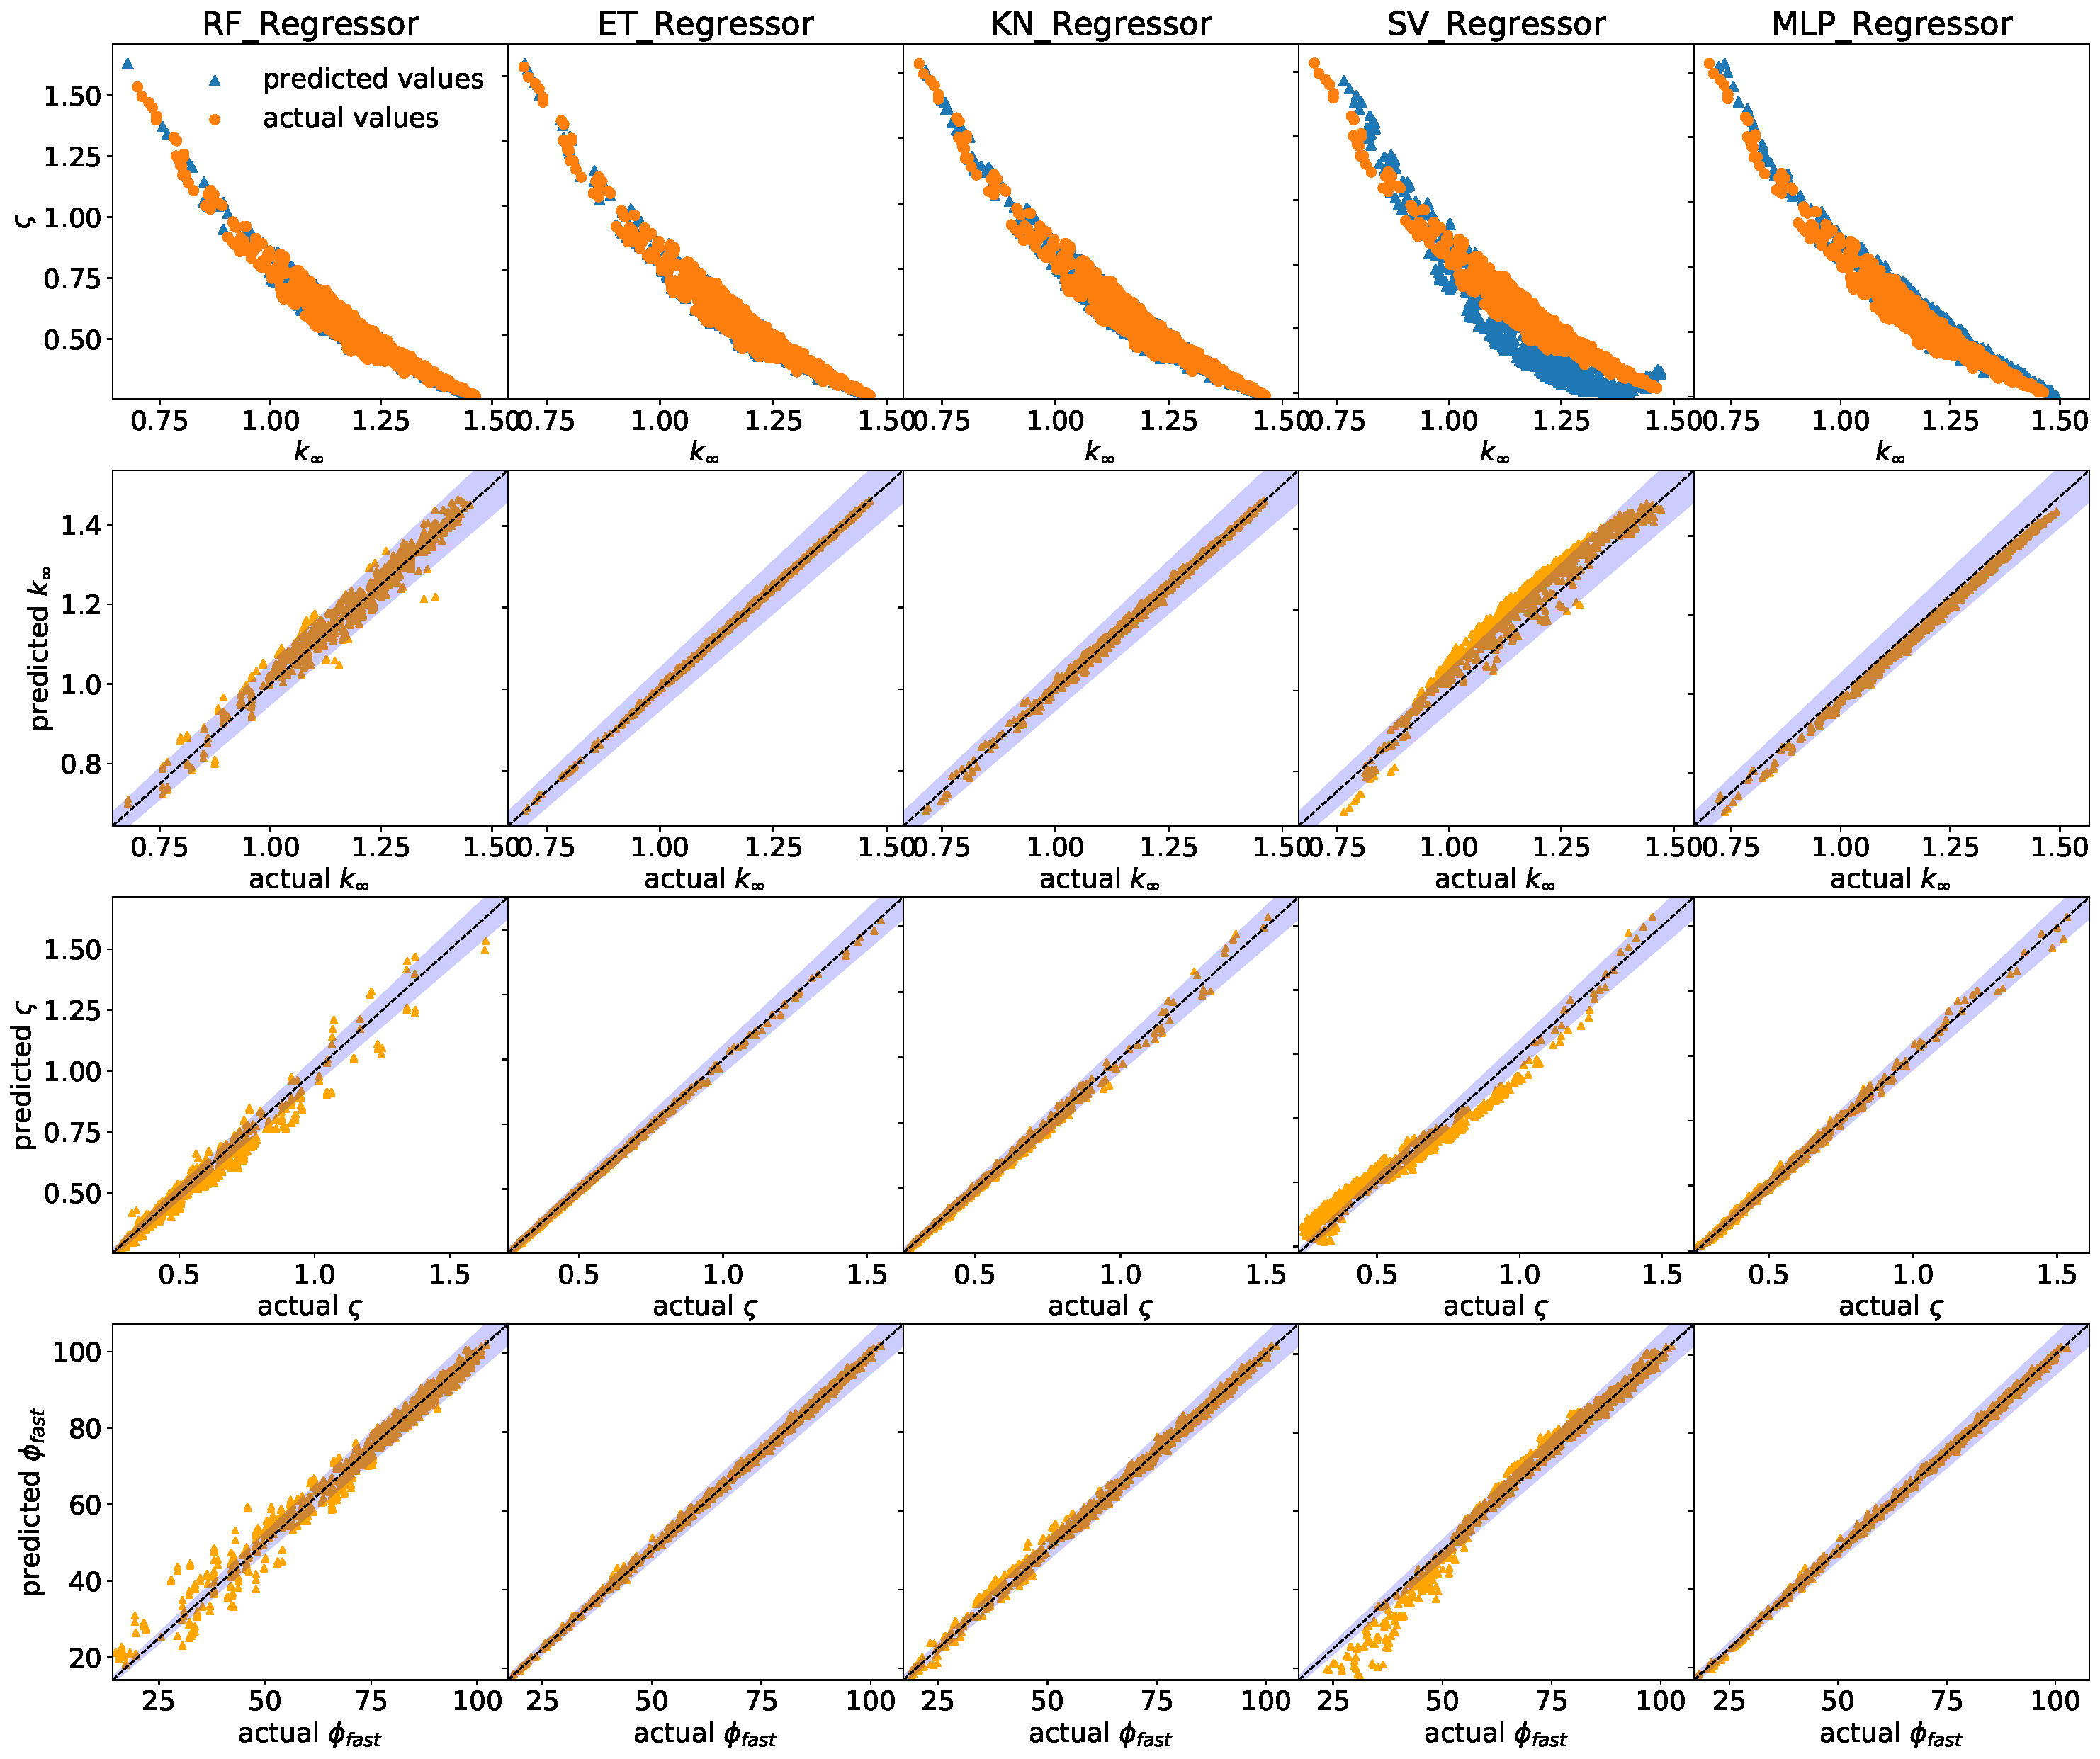
\includegraphics[width=\textwidth]{images/regression_cross_validation.pdf}
     \end{center}
        \caption{Cross-validation plots of the selected regressors, top to bottom:	(i)$k_{\infty}$ versus $\varsigma$ (ii) $k_{\infty}$ (iii) $\varsigma$ and	(iv) $\phi_{fast}$  }
        \label{fig:cv}
    \end{figure}
    \begin{figure}[htbp!]
     \begin{center}
            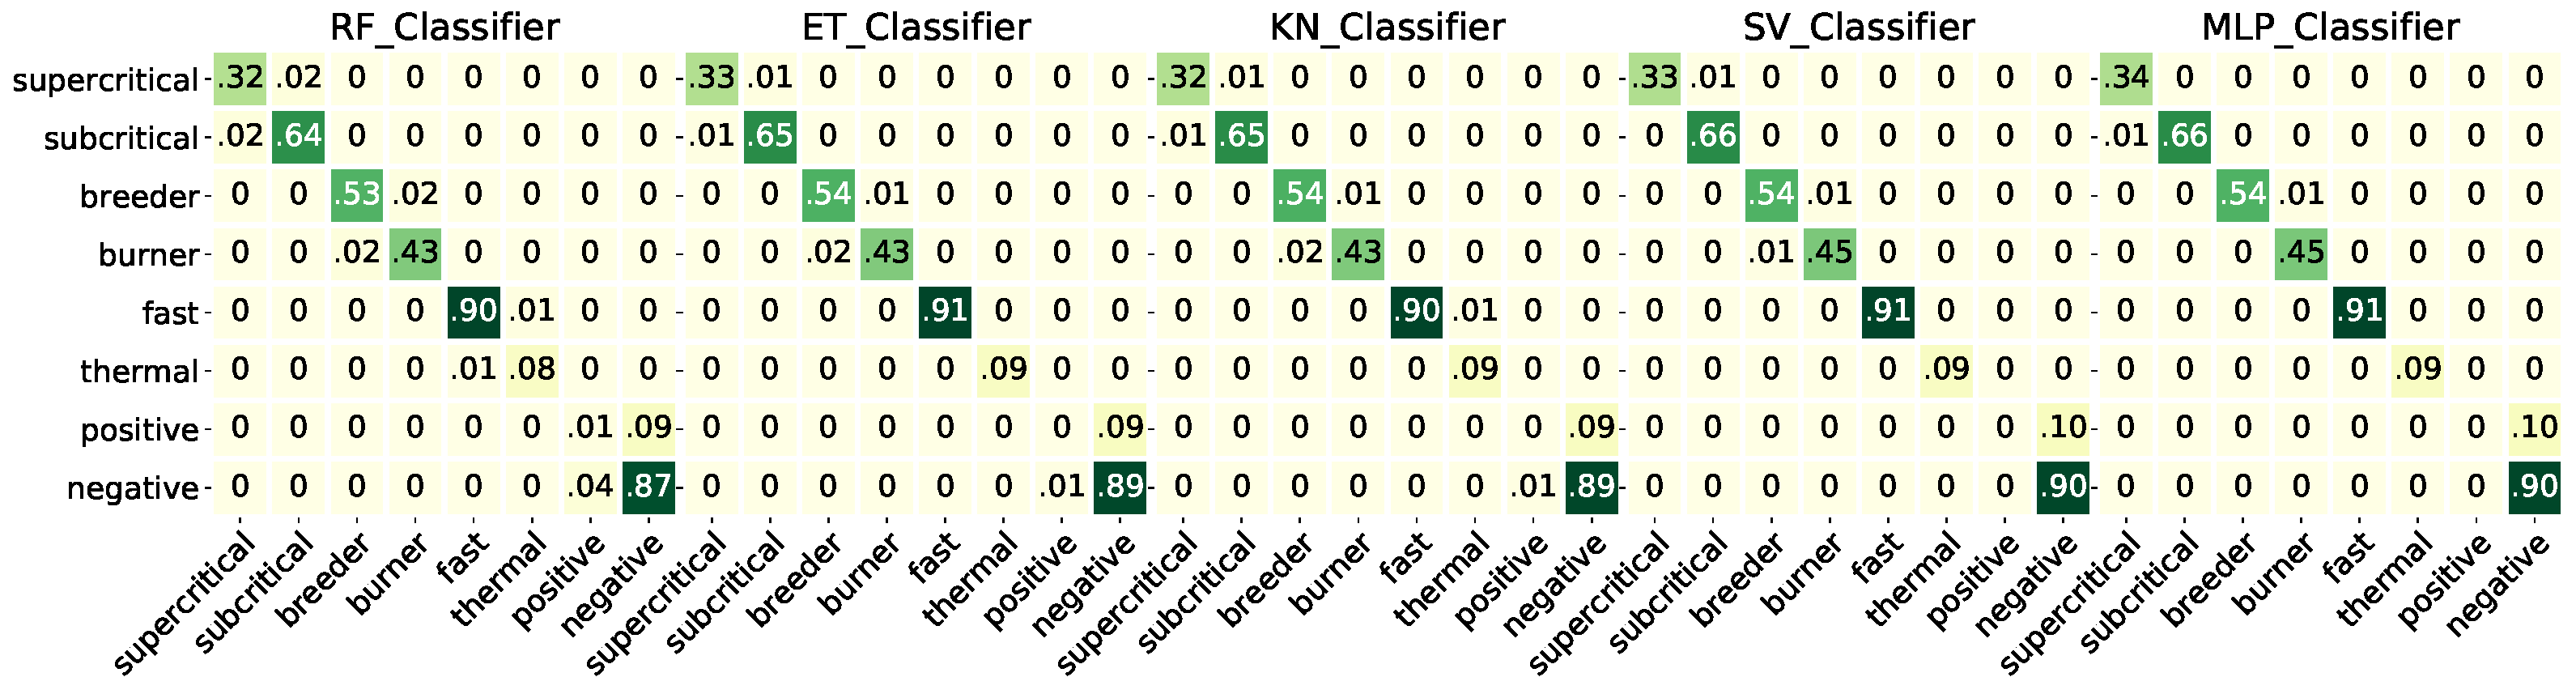
\includegraphics[width=\textwidth]{images/classification_confusion_matrix.pdf}
     \end{center}
        \caption{Normalized confusion matrices of the selected classifiers}
        \label{fig:cm}
    \end{figure}

\subsection{Optimum Designs}
\DIFdelbegin \DIFdel{In accordance with }\DIFdelend \DIFaddbegin

    \DIFadd{Based on }\DIFaddend the constraints applied to \DIFdelbegin \DIFdel{the }\DIFdelend performance metrics, we found a set of optimum solutions for each fuel-salt pair. As an illustration, \DIFdelbegin \DIFdel{Figure~\ref{fig:pareto} depicts the pareto-front }\DIFdelend \DIFaddbegin \DIFadd{we presented the Pareto-front }\DIFaddend solutions for the (U-Th)F$_4$-NaF-BeF$_2$, \DIFaddbegin \DIFadd{which is very }\DIFaddend similar to the results of other fuel-salt pairs\DIFdelbegin \DIFdel{. The
}\DIFdelend \DIFaddbegin \DIFadd{, in Figure~\ref{fig:pareto}. This }\DIFaddend figure includes (a) \DIFdelbegin \DIFdel{the }\DIFdelend cross-validation plots for each performance metric, (b) the distribution of the \DIFdelbegin \DIFdel{pareto-front }\DIFdelend \DIFaddbegin \DIFadd{Pareto-front }\DIFaddend solutions in 3-D performance metric space, and (c) the normalized confusion matrix\DIFdelbegin \DIFdel{for the classification results. From }\DIFdelend \DIFaddbegin \DIFadd{. As seen from }\DIFaddend the subplot (a), the \DIFdelbegin \DIFdel{pareto-optimal }\DIFdelend \DIFaddbegin \DIFadd{Pareto-optimal }\DIFaddend solutions (blue triangle) \DIFdelbegin \DIFdel{overlap }\DIFdelend \DIFaddbegin \DIFadd{overlapped }\DIFaddend very well with the actual values (orange circles)\DIFdelbegin \DIFdel{obtained by the Serpent simulation. Additionally, the solutions show convex distribution in agreement with the
distribution shown in the uppermost subplot of Figure ~\ref{fig:cv}. This
situation can be easily observed from the subplot (b). }\DIFdelend \DIFaddbegin \DIFadd{. }\DIFaddend The other subplots also confirm this situation by showing good distributions in the very proximity of the intersection line of each performance metric.

    The cross-validation subplots also \DIFdelbegin \DIFdel{indicate that }\DIFdelend \DIFaddbegin \DIFadd{indicated that all }\DIFaddend the predicted metrics totally stay within \DIFaddbegin \DIFadd{the }\DIFaddend 5\% relative error (\DIFdelbegin \DIFdel{shaded-area) }\DIFdelend \DIFaddbegin \DIFadd{shaded area) and }\DIFaddend very close to the intersection line. We found even better results for the $k_{\infty}$ \DIFaddbegin \DIFadd{metric }\DIFaddend with no more than 1\% relative error.

    \DIFdelbegin \DIFdel{Like the validation of the solutions obtained by the regression analysis }\DIFdelend \DIFaddbegin \DIFadd{As in the regression analysis results}\DIFaddend , the classification results of the optimal solutions in subplot (c) \DIFdelbegin \DIFdel{, agree }\DIFdelend \DIFaddbegin \DIFadd{agreed }\DIFaddend very well with the actual labels. The only noteworthy complication is the misclassification of a tiny fraction of the feedback indicators. This mislabeling certainly \DIFdelbegin \DIFdel{arises }\DIFdelend \DIFaddbegin \DIFadd{arose }\DIFaddend from the prediction of the ${\alpha_{total}}$ values \DIFaddbegin \DIFadd{as }\DIFaddend discussed before and \DIFdelbegin \DIFdel{are }\DIFdelend \DIFaddbegin \DIFadd{were }\DIFaddend estimated as positive instead of negative. In conformity with the constraints applied to \DIFdelbegin \DIFdel{the }\DIFdelend performance metrics in the optimization phase, all the optimum designs we found are of characteristics of supercritical eigenvalue, fast spectrum, burner type\DIFaddbegin \DIFadd{, }\DIFaddend and negative feedback.

    Of the entire Pareto front solutions (around 650) \DIFdelbegin \DIFdel{accounting }\DIFdelend \DIFaddbegin \DIFadd{which account }\DIFaddend for each combination of the fuel-salt pairs, only the nine best solutions are tabulated in Table~\ref{table:optimaldesigns}. We simply opted for the solutions that grant the highest breeding ratio ($\varsigma$) and the lowest fast flux ($\phi_{fast}$) at the $k_{\infty}$ = 1.06. The only exception for the multiplication factor criterion is for the NaCl salt in U-Pu fuel as \DIFdelbegin \DIFdel{no
}\DIFdelend \DIFaddbegin \DIFadd{there are no solutions with a }\DIFaddend multiplication factor less than 1.21 \DIFdelbegin \DIFdel{has been found }\DIFdelend for this fuel-salt pair.

    \DIFdelbegin \DIFdel{From }\DIFdelend \DIFaddbegin \DIFadd{As provided in }\DIFaddend the table, the suggested solutions can be grouped more easily by fuel type \DIFdelbegin \DIFdel{,
as provided in the table, as the }\DIFdelend \DIFaddbegin \DIFadd{as the }\DIFaddend solutions show a certain relationship with the fuel type rather than \DIFaddbegin \DIFadd{the }\DIFaddend salt type. When \DIFdelbegin \DIFdel{different }\DIFdelend \DIFaddbegin \DIFadd{the }\DIFaddend fuel types are compared to each other, \DIFdelbegin \DIFdel{the }\DIFdelend U-Th \DIFdelbegin \DIFdel{fuel requires }\DIFdelend \DIFaddbegin \DIFadd{fuels require }\DIFaddend the highest $^{235}$U content (18-20\%) due to the existence of the $^{232}$Th isotope which has an absorption cross-section approximately four times higher than $^{238}$U. U \DIFdelbegin \DIFdel{fuel reaches its }\DIFdelend \DIFaddbegin \DIFadd{fuels reach their }\DIFaddend top performance when a moderate amount of $^{235}$U (14-15\%) is used. U-Pu \DIFdelbegin \DIFdel{fuel
needs }\DIFdelend \DIFaddbegin \DIFadd{fuels need }\DIFaddend the lowest amount of $^{235}$U (5\%) as not only does Pu in U-Pu already contain a certain fraction of fissile isotopes like $^{239}$Pu and $^{241}$Pu, but also Pu fissile isotopes emit greater average fission neutrons per absorption. \DIFdelbegin \DIFdel{In a similar way}\DIFdelend \DIFaddbegin \DIFadd{Similarly}\DIFaddend , we noticed that \DIFdelbegin \DIFdel{the }\DIFdelend U-Th \DIFdelbegin \DIFdel{fuel demands about
}\DIFdelend \DIFaddbegin \DIFadd{fuels demand }\DIFaddend 13-14\% Th in U-Th while \DIFdelbegin \DIFdel{the }\DIFdelend U-Pu \DIFdelbegin \DIFdel{fuel favors }\DIFdelend \DIFaddbegin \DIFadd{fuels favor }\DIFaddend the highest grade of U content (90\%).

    A comprehensive look at the common properties of the optimal designs suggests that $T_{ave}$ should be in the range of 1100-1200 K and $\xi$ needs to be at its minimum value \DIFdelbegin \DIFdel{of }\DIFdelend \DIFaddbegin \DIFadd{(}\DIFaddend 0.274\DIFaddbegin \DIFadd{)}\DIFaddend . Furthermore, as expected, Th necessitates higher fissile material than any other fuel \DIFdelbegin \DIFdel{type }\DIFdelend \DIFaddbegin \DIFadd{types }\DIFaddend whereas the fissile material required by the U-Pu fuel is the lowest as the \DIFdelbegin \DIFdel{Pu coming from the }\DIFdelend weapons-grade \DIFdelbegin \DIFdel{already
comprises a great }\DIFdelend \DIFaddbegin \DIFadd{Pu comprises a gread }\DIFaddend deal of fissile isotopes by almost 50\% of its content. On the other hand, unlike \DIFaddbegin \DIFadd{the }\DIFaddend other feature parameters \DIFdelbegin \DIFdel{displaying }\DIFdelend \DIFaddbegin \DIFadd{that display }\DIFaddend a direct characteristic relationship with the fuel type, there is no noticeable evidence to associate the channel-to-channel pitch length ($p$) with the fuel types\DIFdelbegin \DIFdel{but the }\DIFdelend \DIFaddbegin \DIFadd{. The }\DIFaddend $p$ \DIFdelbegin \DIFdel{is
}\DIFdelend \DIFaddbegin \DIFadd{parameter is, however, }\DIFaddend likely to vary with the salt type \DIFdelbegin \DIFdel{. As an example, the NaCl }\DIFdelend \DIFaddbegin \DIFadd{just as the NaCl salt }\DIFaddend calls for a constant pitch value of 1.0 cm in all fuel types.

    \DIFdelbegin \DIFdel{Overall}\DIFdelend \DIFaddbegin \DIFadd{In summary}\DIFaddend , among the \DIFaddbegin \DIFadd{optimal }\DIFaddend designs, it appears that all the fuels mixed with the NaCl salt are the most promising designs. In particular, the \DIFdelbegin \DIFdel{UF}\DIFdelend \DIFaddbegin \DIFadd{F}\DIFaddend $_4$-PuF$_3$-NaCl fuel-salt yields the highest $\varsigma$ and $k_{\infty}$. The most unfavorable side of this fuel-salt is to have a lower ${\alpha_{total}}$ than other salt types but the coefficient is still quite sufficient compared to the \DIFdelbegin \DIFdel{current
}\DIFdelend \DIFaddbegin \DIFadd{exiting }\DIFaddend designs of \gls{MSR}s at the initial state with a total \DIFdelbegin \DIFdel{fuel salt }\DIFdelend \DIFaddbegin \DIFadd{fuel-salt }\DIFaddend feedback coefficient of around -3.4 pcm/K \cite{rykhlevskii2019, robertson1971}. From the reactor safety point of view, \DIFdelbegin \DIFdel{with the highest ${\alpha_{total}}$, the
}\DIFdelend \DIFaddbegin \DIFadd{the }\DIFaddend LiF-BeF$_2$ salt \DIFaddbegin \DIFadd{with the highest ${\alpha_{total}}$ }\DIFaddend is the most favorable.

    \begin{figure*}
    	\begin{center}
    		\begin{minipage}{.49\linewidth}
    			\DIFdelbeginFL %DIFDELCMD < \begin{subfigure}[t]{0.8\linewidth}
%DIFDELCMD < 				%%%
\DIFdelendFL \DIFaddbeginFL \begin{subfigure}[t]{1.0\linewidth}
    				\DIFaddendFL 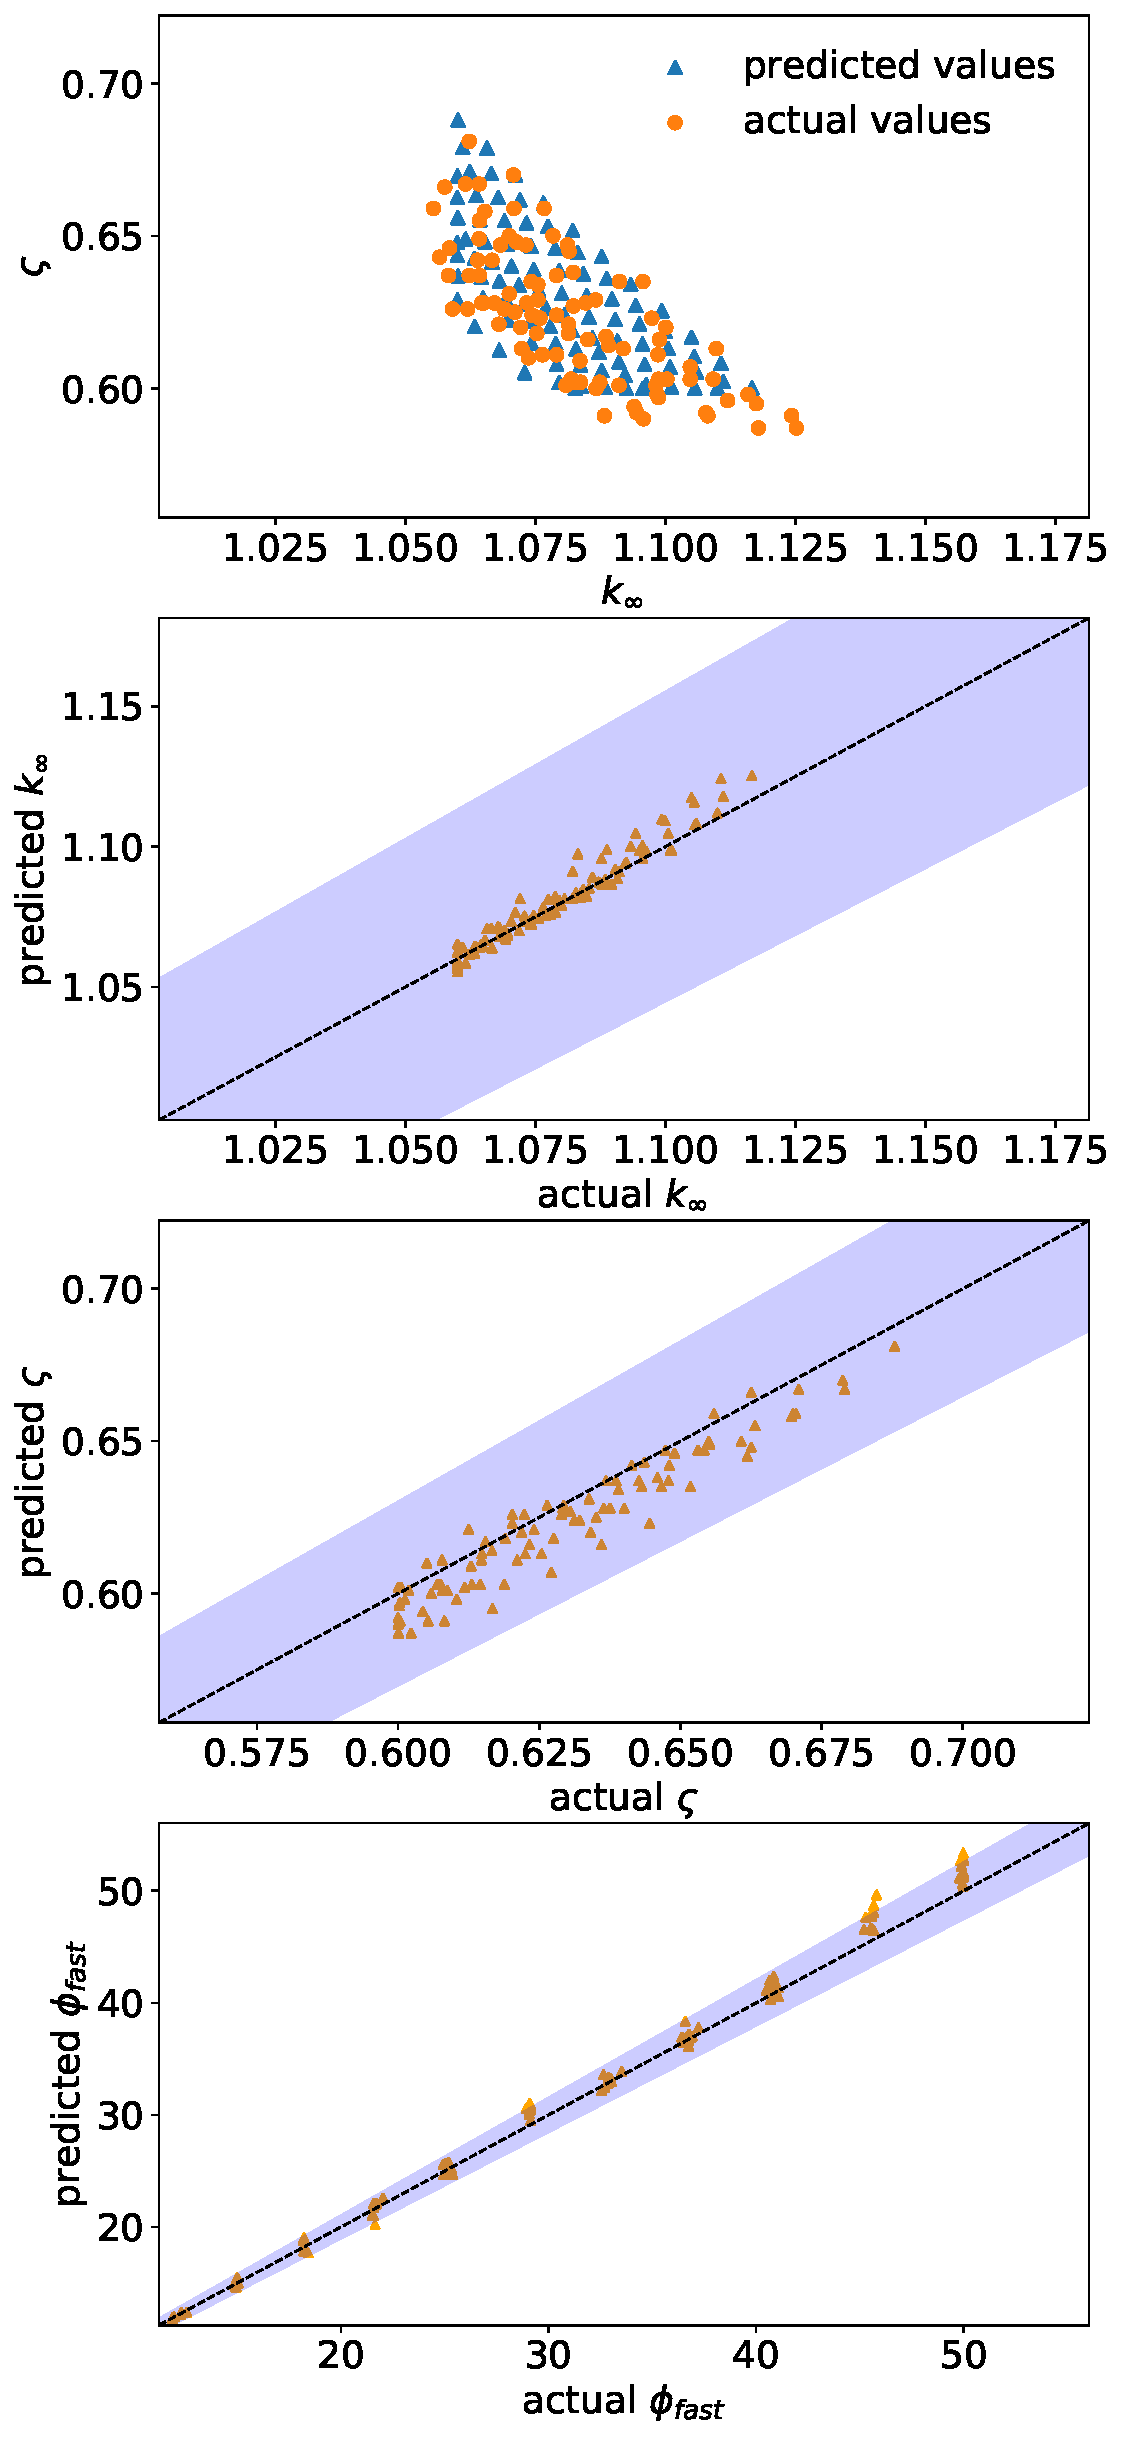
\includegraphics[width=\textwidth]{images/22_optimal_design_cross_validation.pdf}
    				\caption{}
    			\end{subfigure}
    		\end{minipage}
    		\begin{minipage}{.49\linewidth}
    			\DIFdelbeginFL %DIFDELCMD < \begin{subfigure}[t]{0.8\linewidth}
%DIFDELCMD < 				%%%
\DIFdelendFL \DIFaddbeginFL \begin{subfigure}[t]{1.0\linewidth}
    				\DIFaddendFL 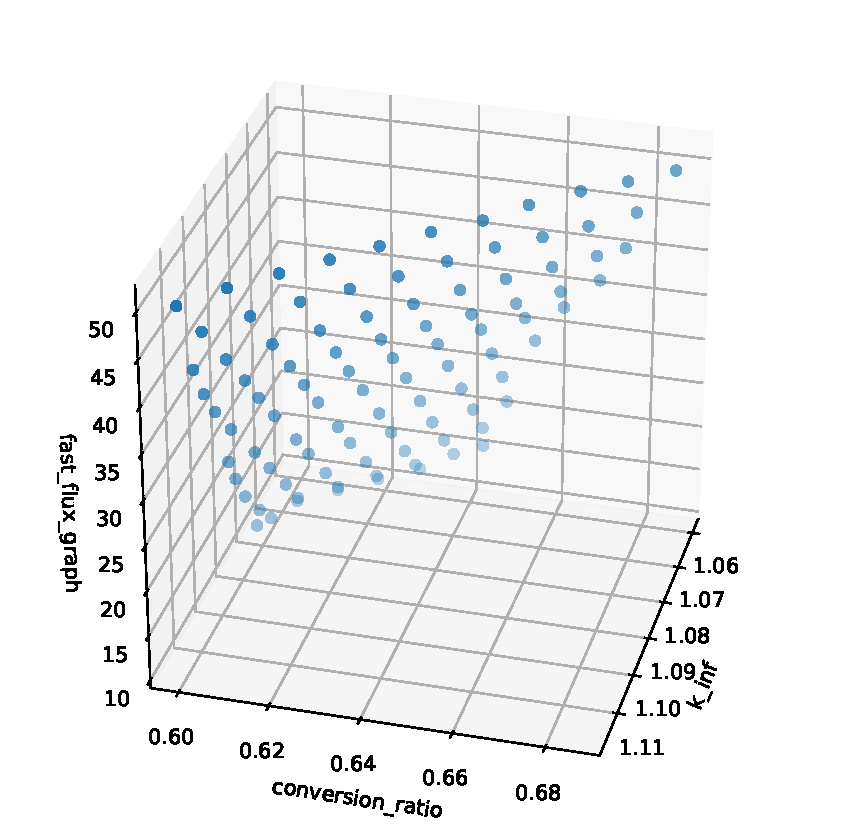
\includegraphics[width=\textwidth]{images/22_optimal_design_3d_solutions.pdf}
    				\caption{}
    			\end{subfigure} \\
    			\DIFdelbeginFL %DIFDELCMD < \begin{subfigure}[b]{0.8\linewidth}
%DIFDELCMD < 				%%%
\DIFdelendFL \DIFaddbeginFL \begin{subfigure}[b]{1.0\linewidth}
    				\DIFaddendFL 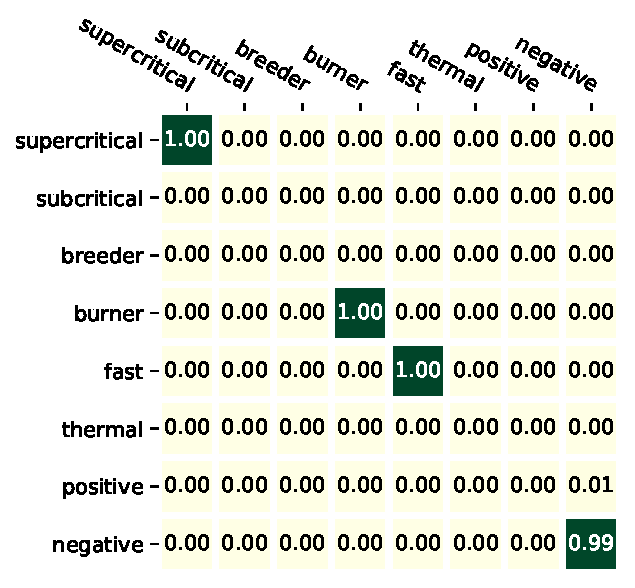
\includegraphics[width=\textwidth]{images/22_optimal_design_confusion_matrix.pdf}
    				\caption{}
    			\end{subfigure}
    		\end{minipage}
    	\end{center}
    	\caption{Optimum solutions for (U-Th)F$_4$-NaF-BeF$_2$: (a) cross-validation plots of performance metrics, (b) \DIFaddbeginFL \DIFaddFL{the }\DIFaddendFL distribution of the \DIFdelbeginFL \DIFdelFL{pareto-front }\DIFdelendFL \DIFaddbeginFL \DIFaddFL{Pareto-front }\DIFaddendFL solutions in 3-D performance metric space, and (c) \DIFaddbeginFL \DIFaddFL{the }\DIFaddendFL normalized confusion matrix.}
    	\label{fig:pareto}
    \end{figure*}


%%%%%%%%%%%%%%%%%%%%%%%%%%%%%%%%%%%%%%%%
\begin{landscape}
	\begin{table}[ht!]
		\centering
		\caption{\DIFdelbeginFL \DIFdelFL{Selected best }\DIFdelendFL \DIFaddbeginFL \DIFaddFL{Optimal }\DIFaddendFL designs for each fuel-salt pair\DIFdelbeginFL %DIFDELCMD < \tnote{$\star$}%%%
\DIFdelendFL \DIFaddbeginFL \DIFaddFL{$^\star$}\DIFaddendFL }
		\begin{threeparttable}[t]
			\begin{tabular}{lllllllllll}
				\hline
				\textbf{Fuel Type} & \textbf{Salt Type}  & \textbf{$f_{35}$} &
				\textbf{$f_{U}$} & \textbf{$p$}	& \textbf{$T_{ave}$} & \textbf{$\xi$} &
				\textbf{$k_{\infty}$ \tnote{$\dagger$}}	& \textbf{$\varsigma$
					\tnote{$\ddagger$}}  & \textbf{$\phi_{fast}$ \tnote{$\perp$}} &
				\textbf{${\alpha_{total}}$ 	\tnote{$\wedge$}}  \\
				\hline

				U 	& LiF-BeF$_2$ 	& 14.47 & 100.0 & 86.7 & 1200 & 0.274 & 1.0600(+60) &
				0.661(-6) & 18.6(-0.5) 	& -3.9\\
				U 	& NaF-BeF$_2$ 	& 14.88 & 100.0 & 7.18 & 1125 & 0.274 & 1.0600(-120) &
				0.638(+6) & 19.0(-0.9) 	& -4.0\\
				U 	& NaCl 	& 14.28 & 100.0 & 1.00 & 1176 & 0.274 & 1.0604(-20) &
				0.692(0) & 12.6(0) 	& -3.0\\
				U-Th & LiF-BeF$_2$ 	& 19.10	& 86.7 & 5.50 & 1123 & 0.276 & 1.0601(-70) &
				0.665(-7) & 17.1(-0.2) 	& -4.3\\
				U-Th & NaF-BeF$_2$ 	& 20.00 & 86.8 & 5.98 & 1125 & 0.275 & 1.0600(+30) &
				0.643(-11) & 16.0(-0.2) & -2.8\\
				U-Th 	& NaCl 	& 18.48	& 86.2 	& 1.00 	& 1199 & 0.274 & 1.0600(+140) 	&
				0.696(-1) & 14.4(0)	& -2.8\\
				U-Pu & LiF-BeF$_2$ 	& 5.00 	& 90.0 	& 4.40 	& 1198 & 0.274 & 1.0600(-20) &
				0.732(+3) & 16.0(0.2) & -4.5\\
				U-Pu	& NaF-BeF$_2$ 	& 5.00 	& 89.3 & 4.37 & 1125 & 0.275 & 1.0600(+460) &
				0.723(+15) & 13.6(0.3) 	& -3.3\\
				U-Pu	& NaCl & 5.00 & 90.0 & 1.00 & 1193 	& 0.274 & 1.2192(+10) &
				0.753(+1) & 13.0(0)	& -3.4\\
				\hline
			\end{tabular}
            \DIFdelbeginFL %DIFDELCMD < \begin{tablenotes}
%DIFDELCMD < 				\item[$\star$] %%%
\DIFdelendFL \DIFaddbeginFL \DIFaddFL{\rule{0in}{1.2em}$^\star$}\scriptsize \DIFaddendFL Performance metrics given in the table are the predicted values. The \DIFdelbeginFL \DIFdelFL{actual values are given within the brackets }\DIFdelendFL \DIFaddbeginFL \DIFaddFL{values inside the brackets are the actual values }\DIFaddendFL in terms of \DIFdelbeginFL \DIFdelFL{differences
				}\DIFdelendFL \DIFaddbeginFL \DIFaddFL{difference }\DIFaddendFL from the predicted values.
\DIFdelbeginFL %DIFDELCMD < \item[$\dagger$] %%%
\DIFdelFL{Computational error of }\DIFdelendFL \DIFaddbeginFL

			\DIFaddFL{\rule{0in}{1.2em}$^\dagger$}\scriptsize \DIFaddFL{The computational error of the }\DIFaddendFL infinite multiplication factor is $\pm$0.0009. The values within the brackets are in the units of pcm.
\DIFdelbeginFL %DIFDELCMD < \item[$\ddagger$] %%%
\DIFdelFL{Computational error of }\DIFdelendFL \DIFaddbeginFL

			\DIFaddFL{\rule{0in}{1.2em}$^\ddagger$}\scriptsize \DIFaddFL{The computational error of the }\DIFaddendFL conversion ratio is $\pm$0.005. The values within the brackets are in the units of milli.
\DIFdelbeginFL %DIFDELCMD < \item[$\perp$] %%%
\DIFdelFL{Computational error of }\DIFdelendFL \DIFaddbeginFL

			\DIFaddFL{\rule{0in}{1.2em}$^\perp$}\scriptsize \DIFaddFL{The computational error of the }\DIFaddendFL fast flux is $\pm$0.007.
\DIFdelbeginFL %DIFDELCMD < \item[$\wedge$] %%%
\DIFdelFL{Propagated }\DIFdelendFL \DIFaddbeginFL

			\DIFaddFL{\rule{0in}{1.2em}$^\wedge$}\scriptsize \DIFaddFL{The propagated }\DIFaddendFL computational error of \DIFaddbeginFL \DIFaddFL{the }\DIFaddendFL feedback coefficient of reactivity is $\pm$0.4.
\DIFdelbeginFL %DIFDELCMD < \end{tablenotes}
%DIFDELCMD < 		%%%
\DIFdelendFL \DIFaddbeginFL

		\DIFaddendFL \end{threeparttable}
		\label{table:optimaldesigns}
	\end{table}
\DIFaddbegin

\DIFaddend \end{landscape}
\DIFaddbegin

\DIFaddend %%%%%%%%%%%%%%%%%%%%%%%%%%%%%%%%%%%%%%%%
